\documentclass[a4paper, 11pt, UTF8]{ctexart}
\usepackage{graphicx}
\usepackage{geometry}
\usepackage{enumerate}
\usepackage{caption}
\usepackage{subfigure}
\usepackage{float}
\usepackage{hyperref}

\hypersetup{hidelinks}


\title{基本功能测试方案}

\author{机械108 \qquad 张益铭 \qquad 2021010552}

\date{\today}

\geometry{left=3cm, right=3cm, top=4cm, bottom=4cm}

\begin{document}

\maketitle

\tableofcontents

\rightline{p.s. 点击目录进行跳转 :)}

\newpage

\section{正常输入}

输入1:123123124132452351345123413521341324*3413241340324123784571932874

输出1:420248937238745134153510177991568300037542274470401219770285176

\begin{figure}[H]
    \centering
    \caption{普通计算}
    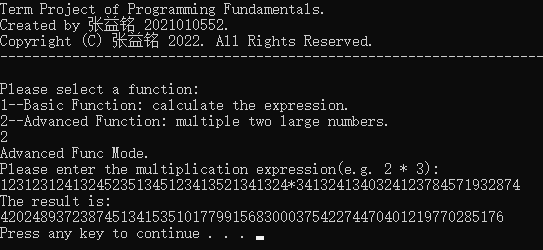
\includegraphics[width=0.8\textwidth]{t2.png}    
\end{figure}

输入2:见图片

输出2:见图片

\begin{figure}[H]
    \centering
    \caption{较长数据测试}
    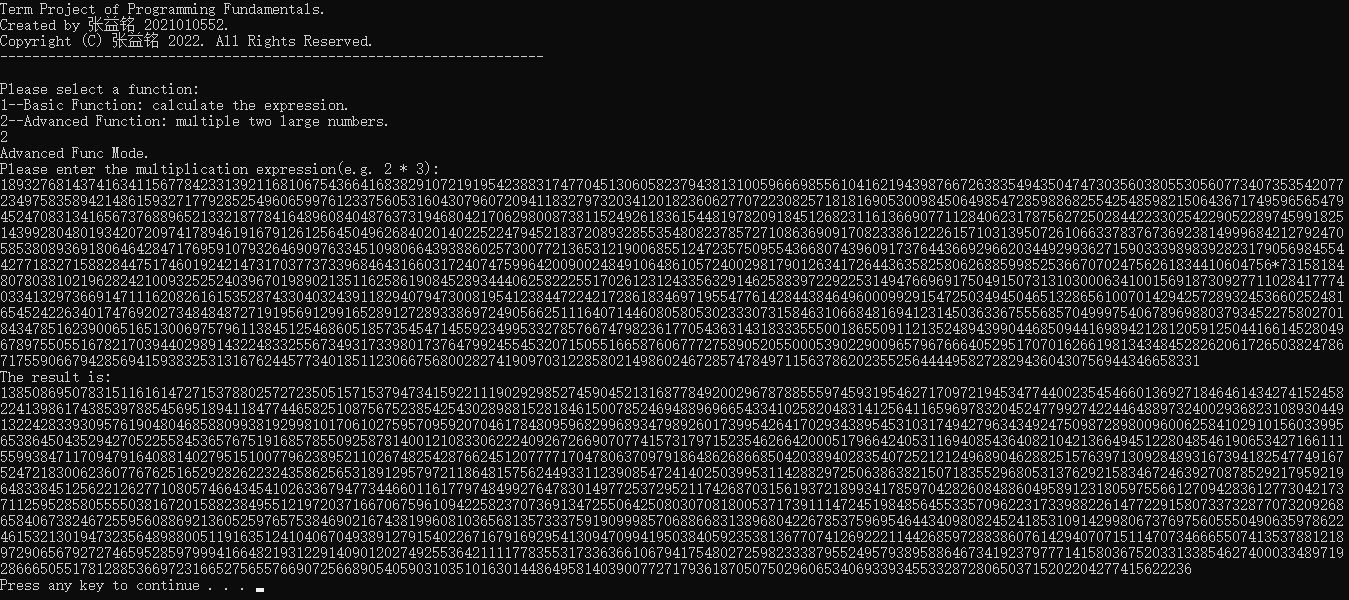
\includegraphics[width=\textwidth]{t1.png}    
\end{figure}

\newpage

\section{鲁棒性测试}

输入3:

输出3:Please enter the expression!

\begin{figure}[H]
    \centering
    \caption{不输入}
    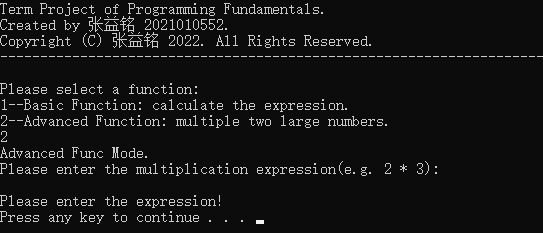
\includegraphics[width=0.8\textwidth]{t3.png}    
\end{figure}

输入4:123 *

输出4:Please enter the second multiplier!

\begin{figure}[H]
    \centering
    \caption{缺少第二个乘数}
    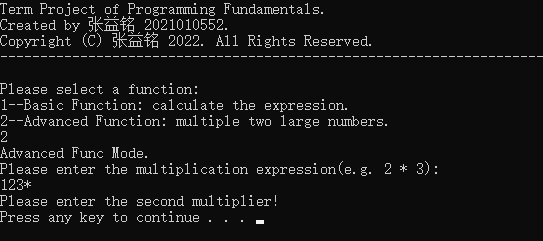
\includegraphics[width=0.8\textwidth]{t4.png}    
\end{figure}

输入5:* 123

输出5:Please enter the first multiplier!

\begin{figure}[H]
    \centering
    \caption{缺少第一个乘数}
    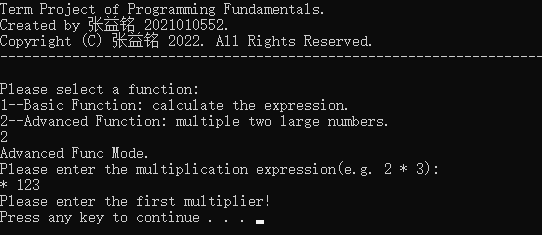
\includegraphics[width=0.8\textwidth]{t5.png}    
\end{figure}

输入6:123 * 456 * 789

输出6:You can ONLY multiply two numbers!

\begin{figure}[H]
    \centering
    \caption{多个数相乘}
    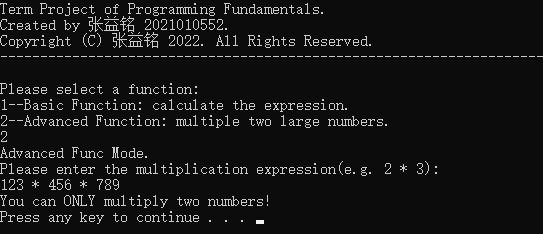
\includegraphics[width=0.8\textwidth]{t6.png}    
\end{figure}

输入7:123 + 456

输出7:You can ONLY enter multiplication signs or numbers!

\begin{figure}[H]
    \centering
    \caption{输入非乘法表达式}
    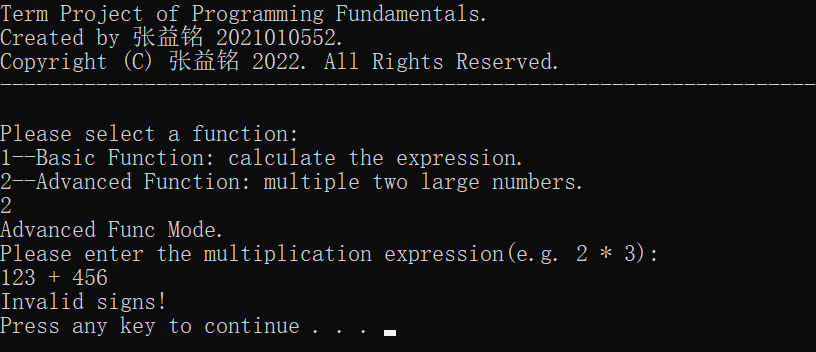
\includegraphics[width=0.8\textwidth]{t7.png}    
\end{figure}

\end{document}